%=============================================================================
% GENERATED FILE -- do not edit.
% Produced by tools/proposal/build_sizing_section.py from the sizing model.
% Every number here is read from rescueswarm_sizing_model or derived from its
% constants and asserted against its result. Edit the model, not this file.
%=============================================================================
\section{Sizing and Analysis}
\label{sec:sizing}

This section shows how we arrived at the design point, not just the result.
Every figure is regenerated from
% \path (url package) rather than \texttt: the path is one unbreakable token
% and overflows an IEEE column by 27 pt in \texttt. \path breaks at the slashes.
\path{tools/sizing-model/rescueswarm_sizing_model.py}, and the section itself is
generated from it, so any change to a constant in the model appears here too.

\subsection{Constants and where they come from}

\begin{center}
\begin{tabular}{@{}llp{4.2cm}@{}}
\toprule
\textbf{Symbol} & \textbf{Value} & \textbf{Basis} \\
\midrule
$\rho$ & 1.150\,kg/m$^3$ & $\sim$30\,\textdegree C at 300\,m density altitude; an Indian summer field, not sea level \\
$\mathrm{FM}$ & 0.60 & Rotor figure of merit, mid-range of the 0.5--0.7 literature band \\
$\eta_{\text{mot}}$ & 0.82 & BLDC efficiency near the hover operating point \\
$\eta_{\text{esc}}$ & 0.95 & Electronic speed controller \\
$P_{\text{avio}}$ & 55\,W & Companion computer, autopilot, GNSS, camera, radios, servos \\
$\mathrm{DoD}$ & 80\% & Usable depth of discharge; land at 20\,\% state of charge \\
$T/W$ & 2.0 & Static thrust-to-weight, a reserve policy \\
\bottomrule
\end{tabular}
\end{center}

We chose two of these values cautiously. Air density is taken for a hot day at
altitude rather than at sea level, which increases the power required, and the
figure of merit is taken from the middle of the published range rather than the
top. We would rather find out now that the design is tight than discover it on
the flying field.

\subsection{Hover power, from momentum theory}

The rotor disk area for 4 rotors of diameter 18\,in
($D=0.4572$\,m) is
\[
\begin{aligned}
A &= N\pi\left(\frac{D}{2}\right)^{2} = 0.6567~\text{m}^2,\\
\text{disk loading} &= \frac{m}{A} = 9.69~\text{kg/m}^2 .
\end{aligned}
\]
Momentum theory gives the induced power needed to produce thrust $T$ over that
disk area~\cite{leishman2006helicopter}. Dividing by the figure of merit
$\mathrm{FM}$, the ratio of ideal induced power to actual shaft power, accounts
for blade drag and uneven inflow and gives the shaft power:
\[
P_{\text{shaft}} = \frac{T^{3/2}}{\mathrm{FM}\sqrt{2\rho A}}
= \frac{(62.4)^{3/2}}{0.60\sqrt{2(1.150)(0.6567)}}
= 668~\text{W},
\]
where $T = mg = 62.4$\,N at the 6.36\,kg maximum take-off mass. Adding
the drivetrain and the avionics load,
\[
P_{\text{elec}} = \frac{P_{\text{shaft}}}{\eta_{\text{mot}}\eta_{\text{esc}}}
+ P_{\text{avio}}
= \frac{668}{0.779} + 55 = 913~\text{W},
\]
which at the 21.6\,V pack nominal is a hover current of
$I = P/V = 42.2$\,A. Power loading is 7.0\,g/W.

\subsection{Peak power and the current the pack must supply}

Induced power scales as $T^{3/2}$, so at the design thrust-to-weight of
2.0 the shaft power rises by $2.0^{3/2}$:
\[
P_{\text{peak}} = \frac{(2.0\,T)^{3/2}}{\mathrm{FM}\sqrt{2\rho A}\,\eta}
+ P_{\text{avio}} = 2481~\text{W}
\;\Longrightarrow\;
I_{\text{peak}} = 114.8~\text{A}.
\]
It is this current, more than the energy, that rules out most candidate packs.
It has to be supplied continuously rather than in short bursts, because the
aircraft must be able to hold 2.0 times its weight, not just reach it
briefly. The modelled pack supplies 135\,A, a margin of 18\,\%,
and each motor's share sets the speed controller rating at 29\,A peak.

This is also why a smaller pack does not work. At 13.5\,Ah the peak is
8.51\,C and hover is 3.13\,C; a pack of half the capacity would need
twice the C-rate to deliver the same current. A larger capacity keeps the
discharge rate down.

\subsection{Propulsion}

\[
\begin{aligned}
T_{\text{total}} &= (T/W)\,mg = 125~\text{N} = 12.72~\text{kgf},\\
T_{\text{motor}} &= 3.18~\text{kgf}.
\end{aligned}
\]
Hover needs 1.59\,kgf per motor, which is 50\,\% of maximum
thrust. This is inside the 45--55\,\% range where both propeller efficiency and
thermal margin are reasonable. Well below that range, the propulsion system
would be larger and heavier than necessary; well above it, there would be too
little thrust left to hold attitude in gusts.

With the motor we have chosen, hover is comfortable but peak thrust is not. The
Tarot TL96020 is rated for 26.5\,A continuous. In hover each motor draws
10.6\,A, which is 40\,\% of that rating. At the design
thrust-to-weight it draws 28.7\,A, or 108\,\%, which is above the
continuous rating. We accept this only because full thrust is a short-term
reserve, not a flight condition: the aircraft hovers at about half throttle and
reaches this current for a few seconds at most, when recovering from a gust or
manoeuvring hard. It is still the tightest margin in the propulsion system, so
the P2 thrust stand measures current as well as thrust to show whether the motor
reaches 3.18\,kgf within its rating. The datasheet also gives a motor mass
of 168\,g, compared with the 160\,g the sizing model assumes, a
difference of +32\,g per aircraft that we will confirm when we weigh the
parts in P5.

\subsection{The coupled mass and energy solve}

Pack mass, take-off mass and mission energy all depend on one another: a heavier
pack raises hover power, which raises the energy needed, which raises the pack
mass again. The model repeats the calculation until the values settle.

The reserve is what fixes the result. The pack must provide enough usable energy
for the mission, one complete second sweep of the search area, and four minutes
of hovering:
\[
\underbrace{103.4}_{\text{nominal}} + \underbrace{30.9}_{\text{re-sweep}}
+ \underbrace{60.8}_{\text{loiter}} = 195.2~\text{Wh usable},
\]
against 233.3\,Wh available at 80\% depth of discharge, a margin of
19\,\%. Whatever its chemistry, a candidate pack must therefore be rated
for at least \textbf{244\,Wh} at \textbf{6S} and supply
\textbf{114.8\,A continuously}.

The model was sized with 18 cells in 6S3P:
292\,Wh, 13.5\,Ah, 1449\,g, 21.6\,V nominal
(18--25.2\,V). Hover endurance is 15.3\,min against a
7.6\,min design mission consuming 103.4\,Wh. The pack now specified
is a bought 6S 16\,Ah LiPo (Section~\ref{sec:energy}); these figures are
re-run on its measured mass before first flight.

At 6.36\,kg per aircraft the fleet weighs 19.08\,kg, against the
25.0\,kg regulatory limit, a margin of 24\,\%.

\subsection{Camera and optics}

All of the optics follow from three numbers: pixel count, pixel size and focal
length. The active sensor area is the pixel count times the pixel size,
\[
\begin{aligned}
w &= 4056 \times 1.55\,\text{\textmu m} = 6.287~\text{mm},\\
h &= 4.712~\text{mm}, \qquad d = 7.86~\text{mm},
\end{aligned}
\]
and the fields of view are calculated exactly, without the small-angle
approximation:
\[
\begin{aligned}
\theta &= 2\arctan\!\left(\frac{s}{2f}\right)\\
&\Rightarrow\;
\text{HFOV}=55.3^\circ,\;
\text{VFOV}=42.9^\circ,\;
\text{DFOV}=66.4^\circ .
\end{aligned}
\]
By similar triangles through the lens, the ground sample distance at altitude
$H$ is
\[
\text{GSD} = \frac{p\,H}{f}
= \frac{1.55\,\text{\textmu m}\times 40\,\text{m}}{6\,\text{mm}}
= 1.03~\text{cm/px},
\]
giving a 41.9\,$\times$\,31.4\,m footprint. One pixel subtends
14.80\,mdeg.

We consider two target sizes and design for the smaller one. An adult 1.7\,m
tall lying on a rooftop or dry ground covers 165\,px, or
7,960\,px$^2$. A person in water shows only head and shoulders, about
0.4\,m across, and covers 39\,px, or 1,498\,px$^2$, roughly a
quarter of the area. We design for the person in water, because this is a flood
system and that is the posture we expect. The larger figure is the easy case and
is given only for comparison. Section~\ref{sec:perception} bases the tiling
decision on the water figure.

\textit{Focus} is not a problem. The hyperfocal distance,
\[
H_{\text{hyp}} = \frac{f^{2}}{Nc} + f = 4.15~\text{m},
\]
taking the circle of confusion as two pixels, puts everything from
2.08\,m to infinity in acceptable focus. The aircraft never flies below
30\,m, so a fixed lens set once is in focus at every altitude we use. A focusing
mechanism would only add a moving part, extra power draw and a failure we could
not detect in flight.

\textit{Motion blur} is not a limit either. Keeping blur under one pixel
requires $t_{\text{exp}} \le \text{GSD}/v$, which at 8\,m/s is
1.29\,ms, a shutter speed of $1/774$\,s. We already require
$1/1000$\,s or faster.

\textit{Rolling shutter} has a small effect. Reading out the frame takes
25\,ms, during which the aircraft moves, giving 0.20\,m of skew from top
to bottom, about 19\,px. This does not matter for detection, but it does
matter for geolocation: unless the software corrects for the row in which a
detection appears, its position will be biased along the direction of flight.

\textit{Number of views} is where the budget falls short. A target stays in the
frame for the footprint length divided by ground speed, so at 40\,m and 2\,Hz it
is seen 7.9 times, against the 12 views we want for combining
frames. Getting that many needs
\[
r \ge \frac{n\,v}{D} = 3.06~\text{Hz},
\]
The options are a faster capture rate, a lower ground speed, a higher altitude,
or accepting fewer views. Raising the capture rate is the cheapest. Flying lower
shrinks the footprint faster than it shortens the pass, so it actually increases
the rate needed; flying higher makes the ground resolution coarser; and flying
slower makes every pass longer.

The cost of a faster capture rate is processing, not energy. At 48 tiles
per frame it needs 147 detector runs per second, against the
130--160 per second measured for the accelerator, which is at or beyond its
limit. A two-stage approach could recover this. A first stage that only asks
whether a tile is plain open water is judging texture, not looking for a person,
so it still works on a shrunken image even though, as
Section~\ref{sec:perception} shows, a person would be lost at that size. At
$96\times96$ input it handles about 44 times fewer pixels than the
detector, and discarding the open-water tiles would leave the equivalent of
about 22 full detector runs. This first stage would run on the
accelerator we already carry rather than on an extra processor, because the
saving is in detector runs, not power: computing uses less than one per cent of
the aircraft's hover power.

\subsection{Payload release ballistics}

A kit of 200\,g tumbling with drag coefficient 1.05 and reference area
117\,cm$^2$ has ballistic coefficient
$\beta = m/(C_dA) = 16.3$\,kg/m$^2$ and terminal velocity
\[
v_{\text{term}} = \sqrt{\frac{2mg}{\rho C_d A}} = 16.2~\text{m/s}.
\]
Integrating the fall with quadratic drag from a 6\,m release gives
1.15\,s to impact at 9.7\,m/s, with a crosswind drift of 3.24\,m at
3\,m/s and 6.13\,m at 6\,m/s.

The speed of the aircraft at release matters far more than the height. A
remaining ground speed of 0.5\,m/s moves the impact point by about 0.53\,m,
while a whole metre of height error moves it by less than 4\,cm. This is why we
hover before dropping: a multirotor can stop before release, and a fixed-wing
aircraft cannot.

\subsection{Structure, geometry and control authority}

Tip clearance of 30\,mm between adjacent 18\,in rotors sets a diagonal
wheelbase of 689\,mm and an arm length of 0.345\,m. At the design
thrust-to-weight the root bending moment is
\[
\mathcal{M} = T_{\text{motor}}\,L = 10.7~\text{N}\,\text{m}.
\]
For a 25\,$\times$\,23\,mm carbon tube,
$I = \pi(D_o^4 - D_i^4)/64 = 5438$\,mm$^4$, so the bending stress is
$\sigma = \mathcal{M}c/I = 25$\,MPa against roughly 600\,MPa for
unidirectional carbon, a safety factor of about 24.

Bending is therefore not what limits the structure, and we should not design as
if it were. The joints and clamps, and vibration fatigue where the arm meets the
frame, matter much more. A tube that passes the bending case by a factor of
24 is being chosen for stiffness and ease of handling, not strength.

Dropping one kit from a magazine that sits off the centreline moves the centre
of gravity by less than 2\,mm, which takes only a few tens of grams of extra
thrust to correct. The amount is tiny, but it happens suddenly and disturbs the
attitude control. We avoid this by mounting the magazine on the centre of
gravity and holding position briefly after each release.

\subsection{Radio links}
\label{sec:links}

Three kinds of traffic have to be carried, and they have very different needs.
Video needs a high data rate but can be lost occasionally. Command and abort need
little data but must not be lost. Mission data and coordination also need little
data and must keep working even when the other two fail. We first planned to
carry all three on one 5.8\,GHz 802.11 mesh network, but dropped the idea after
working out its link budget.

\subsubsection{Link margin}

Free-space path loss at the 600\,m design slant range follows Friis,
\begin{equation}
\mathrm{FSPL} = 20\log_{10}\!\left(\frac{d}{1\,\text{km}}\right)
              + 20\log_{10}\!\left(\frac{f}{1\,\text{MHz}}\right) + 32.44 ,
\label{eq:fspl}
\end{equation}
but path loss alone does not tell us much, since it is always higher at
5.8\,GHz than at 865\,MHz. What decides whether a link works is the margin left
over,
\begin{equation}
M = P_{\mathrm{tx}} + G_{\mathrm{tx}} + G_{\mathrm{rx}}
    - \mathrm{FSPL}(f,d) - S_{\mathrm{rx}} ,
\label{eq:margin}
\end{equation}
where $S_{\mathrm{rx}}$ is the receiver sensitivity for the modulation we
actually use, not the best figure on the datasheet. Table~\ref{tab:links} gives
(\ref{eq:margin}) at the geofence for our three links.

\begin{table}[t]
\caption{Adopted radio links, evaluated at the 600\,m geofence}
\label{tab:links}
\centering
\small
\setlength{\tabcolsep}{4pt}
\begin{tabular}{@{}lrrrrr@{}}
\toprule
 & $P_{\mathrm{tx}}$ & $\Sigma G$ & $S_{\mathrm{rx}}$ & FSPL & $M$ \\
\textbf{Link} & (dBm) & (dBi) & (dBm) & (dB) & (dB) \\
\midrule
Digital video, 5.8\,GHz & 27.0 & 20 & $-86$ & 103.3 & \textbf{29.7} \\
ExpressLRS, 2.4\,GHz & 20.0 & 4 & $-108$ & 95.6 & \textbf{36.4} \\
LoRa, 865\,MHz SF7 & 14.0 & 4 & $-123$ & 86.7 & \textbf{54.3} \\
\bottomrule
\end{tabular}
\end{table}

\subsubsection{Why we dropped the single mesh}

Applying (\ref{eq:margin}) to the 802.11 setup we had planned, with 20\,dBm into
5\,dBi antennas at each end and an MCS0 sensitivity of $-82$\,dBm, the same
103.3\,dB of path loss leaves only 8.7\,dB of margin. That would have
been the weakest link in the system and also the one carrying the most data, so
the link most likely to fail would also be the one whose failure costs most.
With three separate radios, every link has more than 29.7\,dB, an
improvement of 21.0\,dB on the video link alone (Fig.~\ref{fig:links}a).

A mesh does not solve this, even though that was the original reason for
choosing one. Relaying through a second aircraft replaces one 600\,m link with
two shorter ones and reduces path loss. But each hop uses the same radio,
antennas and sensitivity, so the relay is only as reliable as the aircraft
carrying it, and the things that break the direct link, such as a banked
airframe, a person between the antennas or rain, tend to affect both hops. A
mesh improves average throughput but not the worst case, and the worst case was
our problem.

The 802.11 link would not be useless. It only reaches its sensitivity limit at
1.64\,km and would work well in good conditions (Fig.~\ref{fig:links}b).
But rain, people in the way, a banked airframe and misaligned antennas all eat
into the margin, none of them is included in (\ref{eq:margin}), and
8.7\,dB is not enough to cover them. Our video link has 29.7\,dB at
the same distance and only runs out at 18.4\,km.

\begin{figure*}[t]
\centering
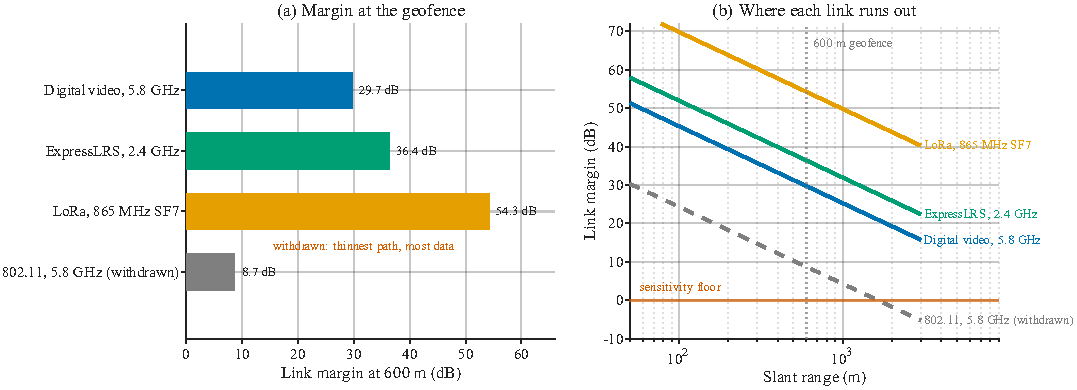
\includegraphics[width=\textwidth]{fig-links.pdf}
\caption{(a) Link margin at the 600\,m geofence, from (\ref{eq:margin}). The
802.11 mesh we dropped is included for comparison. (b) Margin against distance.
Each of our links is used at a small fraction of its maximum range; the dropped
mesh would not have been.}
\label{fig:links}
\end{figure*}

\subsubsection{Sizing the coordination channel}

Splitting the links has a consequence that the margin table does not show. The
mesh would have offered about 235\,kbps of non-video capacity per
aircraft, whereas LoRa at SF7 on a 125\,kHz channel carries 5469\,bps
for the whole fleet, 129 times less. We had not compared the two designs
against the same traffic, so at first we missed this.

What matters is time on air, not bit rate. For the short packets this mission
sends, LoRa's preamble and header take up most of the time. The number of
symbols in a packet of $\mathit{PL}$ bytes is
\begin{equation}
n_{\mathrm{sym}} = n_{\mathrm{pre}} + 4.25 + 8 +
\left\lceil \frac{8\mathit{PL} - 4\mathrm{SF} + 44}{4\,\mathrm{SF}} \right\rceil
(\mathrm{CR}+4),
\label{eq:airtime}
\end{equation}
each lasting $2^{\mathrm{SF}}/\mathrm{BW}$. A 36-byte message therefore
takes 77.1\,ms on air, compared with the 52.7\,ms its data alone
would suggest, so the overhead is about a third of the total.

Our first plan sent aircraft state, task coordination and detection reports as
three separate messages, each at its own rate. That meant three preambles and
three headers per aircraft per second, and it used 28.4\,\% of the
channel, more than the 25\,\% limit we set to leave room for retries and
a fourth node. Combining them into one 36-byte message per aircraft per
second, with a detection added when there is one, brings this down to
25.3\,\%. That still leaves almost no spare capacity: the maximum message
rate is 1.0\,Hz against the 1\,Hz we need.

The answer is already in Table~\ref{tab:links}. The 865\,MHz link has 54.3\,dB
of margin at the geofence, far more than this mission needs; the spreading
factor is buying range we do not use. The SX1262 can also run GFSK with the same
chip, antennas and 14\,dBm output. At 50\,kbps its sensitivity is
$-104$\,dBm instead of $-123$\,dBm, which gives up 19\,dB of the
spare margin for a 9.1 times higher data rate. Each message then takes
7.8\,ms, channel use drops to 2.3\,\%, and the margin is still
35.3\,dB, more than the video link has, while using only a tenth of
the channel.

\begin{table}[t]
\caption{Coordination channel, three aircraft, one 36\,B frame each at 1\,Hz}
\label{tab:coord}
\centering
\small
\begin{tabular}{@{}lrrrr@{}}
\toprule
\textbf{Mode} & \textbf{Rate} & \textbf{Frame} & \textbf{Occupancy} & \textbf{Margin} \\
\midrule
GFSK 50\,kbps      & 50\,kbps & 7.8\,ms & \textbf{2.3\,\%} & 35.3\,dB \\
LoRa SF7, 125\,kHz & 5.5\,kbps & 84.2\,ms & 25.3\,\% & 54.3\,dB \\
\bottomrule
\end{tabular}
\end{table}

We therefore use GFSK normally and LoRa SF7 as a fallback, switching on the same
radio without any hardware change. The fallback is genuinely slower: at
25.3\,\% channel use it supports only 1.0\,Hz, so when we switch
to it we lower the message rate.

\subsubsection{Order of degradation}

We have arranged the links so that they fail in a sensible order, following
their margins. Video is allowed to fail first. Because it is digital, the picture
stays clean until the margin runs out and then frames start to drop, and losing
it costs the operator a view but does not affect the aircraft's decisions.
Coordination degrades next, from GFSK to LoRa SF7 and then to a lower message
rate. Command and abort come last, on ExpressLRS with 36.4\,dB of margin,
and are never traded away: if that link is lost, the aircraft carries out its
failsafe rather than waiting for the link to return. All the bands are
licence-free in India: the 865--867\,MHz short-range device band for
coordination, and the 2.4 and 5.8\,GHz ISM bands for command and video, each
used well within its power limit.

There are two limitations. All these margins assume free space, so they are best
cases: reflections off water, a low ground antenna clipping the Fresnel zone,
and the airframe blocking the signal in a turn all happen in practice and none
is modelled. And the GFSK sensitivity comes from the datasheet, not a
measurement. In P5 we will measure packet loss against distance on the built
aircraft, and only then will Table~\ref{tab:coord} be backed by evidence.

\subsection{Limits of this section}

Every figure in this section is modelled. The thrust figures rely on a motor
with no published thrust curve, and the detection figures assume a recall that
has not been measured. The sizing is consistent and its arithmetic can be
checked, but that does not show that the aircraft can actually do these things,
and we do not claim that it can.
